W niniejszym rozdziale przedstawiono podstawy teoretyczne architektur systemów informatycznych istotnych z punktu widzenia dalszej części pracy, tj. architektury monolitycznej oraz architektury mikroserwisowej. Omówiono ich najważniejsze cechy, typowe zalety i ograniczenia, a także konsekwencje wyboru danego stylu architektonicznego dla wydajności, skalowalności oraz kosztów utrzymania systemu. Szczególną uwagę poświęcono komunikacji między usługami, ponieważ w części eksperymentalnej pracy analizowany jest wariant mikroserwisowy wykorzystujący komunikację gRPC. Przegląd ten stanowi podstawę do zrozumienia kompromisów projektowych występujących przy budowie aplikacji monolitycznych oraz rozproszonych \cite{tapia2020monolithic,blinowski2022monolithic,okroj2023differences,berry2024migrating,bernsteiner2025performance}.

\section{Architektura monolityczna}
\label{sec:monolithic-architecture}

Architektura monolityczna jest klasycznym sposobem budowy aplikacji serwerowych. W takim podejściu logika biznesowa, warstwa dostępu do danych oraz interfejs aplikacyjny pozostają częścią jednego wdrażalnego artefaktu uruchamianego jako pojedynczy proces lub zestaw identycznych instancji tej samej aplikacji. Poszczególne moduły mogą być logicznie wydzielone w kodzie, jednak z perspektywy wdrożeniowej i operacyjnej system funkcjonuje jako całość \cite{tapia2020monolithic,blinowski2022monolithic,benavente2022comparative,mangwani2023evaluation,nayim2023ecommerce}.

W praktyce monolit często korzysta ze wspólnej bazy danych i jednolitego procesu budowania oraz wdrażania. Takie podejście redukuje liczbę elementów infrastrukturalnych, ale równocześnie powoduje, że zmiany w jednej części systemu mogą wymagać przebudowy i ponownego wdrożenia całej aplikacji. W literaturze architektura monolityczna jest opisywana jako rozwiązanie szczególnie korzystne na wczesnych etapach rozwoju produktu lub w projektach o umiarkowanej złożoności, gdzie kluczowe znaczenie mają prostota organizacyjna, krótki czas wdrożenia i niski narzut operacyjny \cite{villamizar2017cost,tapia2020monolithic,blinowski2022monolithic,okroj2023differences,berry2024migrating}.

\subsection{Cechy charakterystyczne architektury monolitycznej}
\label{subsec:monolith-characteristics}

Najbardziej charakterystyczną cechą monolitu jest ścisłe współistnienie wszystkich warstw systemu w jednym artefakcie wykonywalnym. Oznacza to, że interfejs aplikacyjny, logika biznesowa i dostęp do danych są wdrażane oraz wersjonowane razem. Taki model sprzyja spójności rozwiązania i upraszcza zarządzanie zależnościami, lecz jednocześnie zmniejsza autonomię poszczególnych części systemu \cite{tapia2020monolithic,blinowski2022monolithic,benavente2022comparative}.

Drugą ważną cechą jest komunikacja wewnętrzna realizowana lokalnie, najczęściej przez bezpośrednie wywołania metod lub funkcji. Brak konieczności przesyłania danych przez sieć ogranicza narzut serializacji, deserializacji, trasowania i obsługi zdalnych błędów. W konsekwencji monolit może osiągać dobre wyniki wydajnościowe w scenariuszach, w których duża część logiki wykonywana jest w ramach jednego procesu \cite{tapia2020monolithic,blinowski2022monolithic,okroj2023differences,bernsteiner2025performance}.

Kolejną cechą jest scentralizowany model wdrożenia. Zmiana w pojedynczym module nie jest wdrażana niezależnie, lecz staje się częścią nowej wersji całej aplikacji. Taki sposób pracy upraszcza zarządzanie wersjami, ale w miarę wzrostu systemu prowadzi do silniejszego sprzężenia zespołów, dłuższych cykli integracyjnych i większego ryzyka regresji przy wdrożeniach \cite{mangwani2023evaluation,nayim2023ecommerce,berry2024migrating}.

Na rysunku~\ref{fig:chapter2-monolith-vs-microservices} przedstawiono przykładowe ujęcie porównawcze architektury monolitycznej i mikroserwisowej. W przypadku monolitu warstwa interfejsu użytkownika, logiki biznesowej oraz dostępu do danych stanowią element jednego systemu, który współpracuje ze wspólnym magazynem danych. Tego rodzaju układ dobrze oddaje podstawową ideę monolitu jako jednolitego, centralnie zarządzanego rozwiązania.

\begin{figure}[htbp]
    \centering
    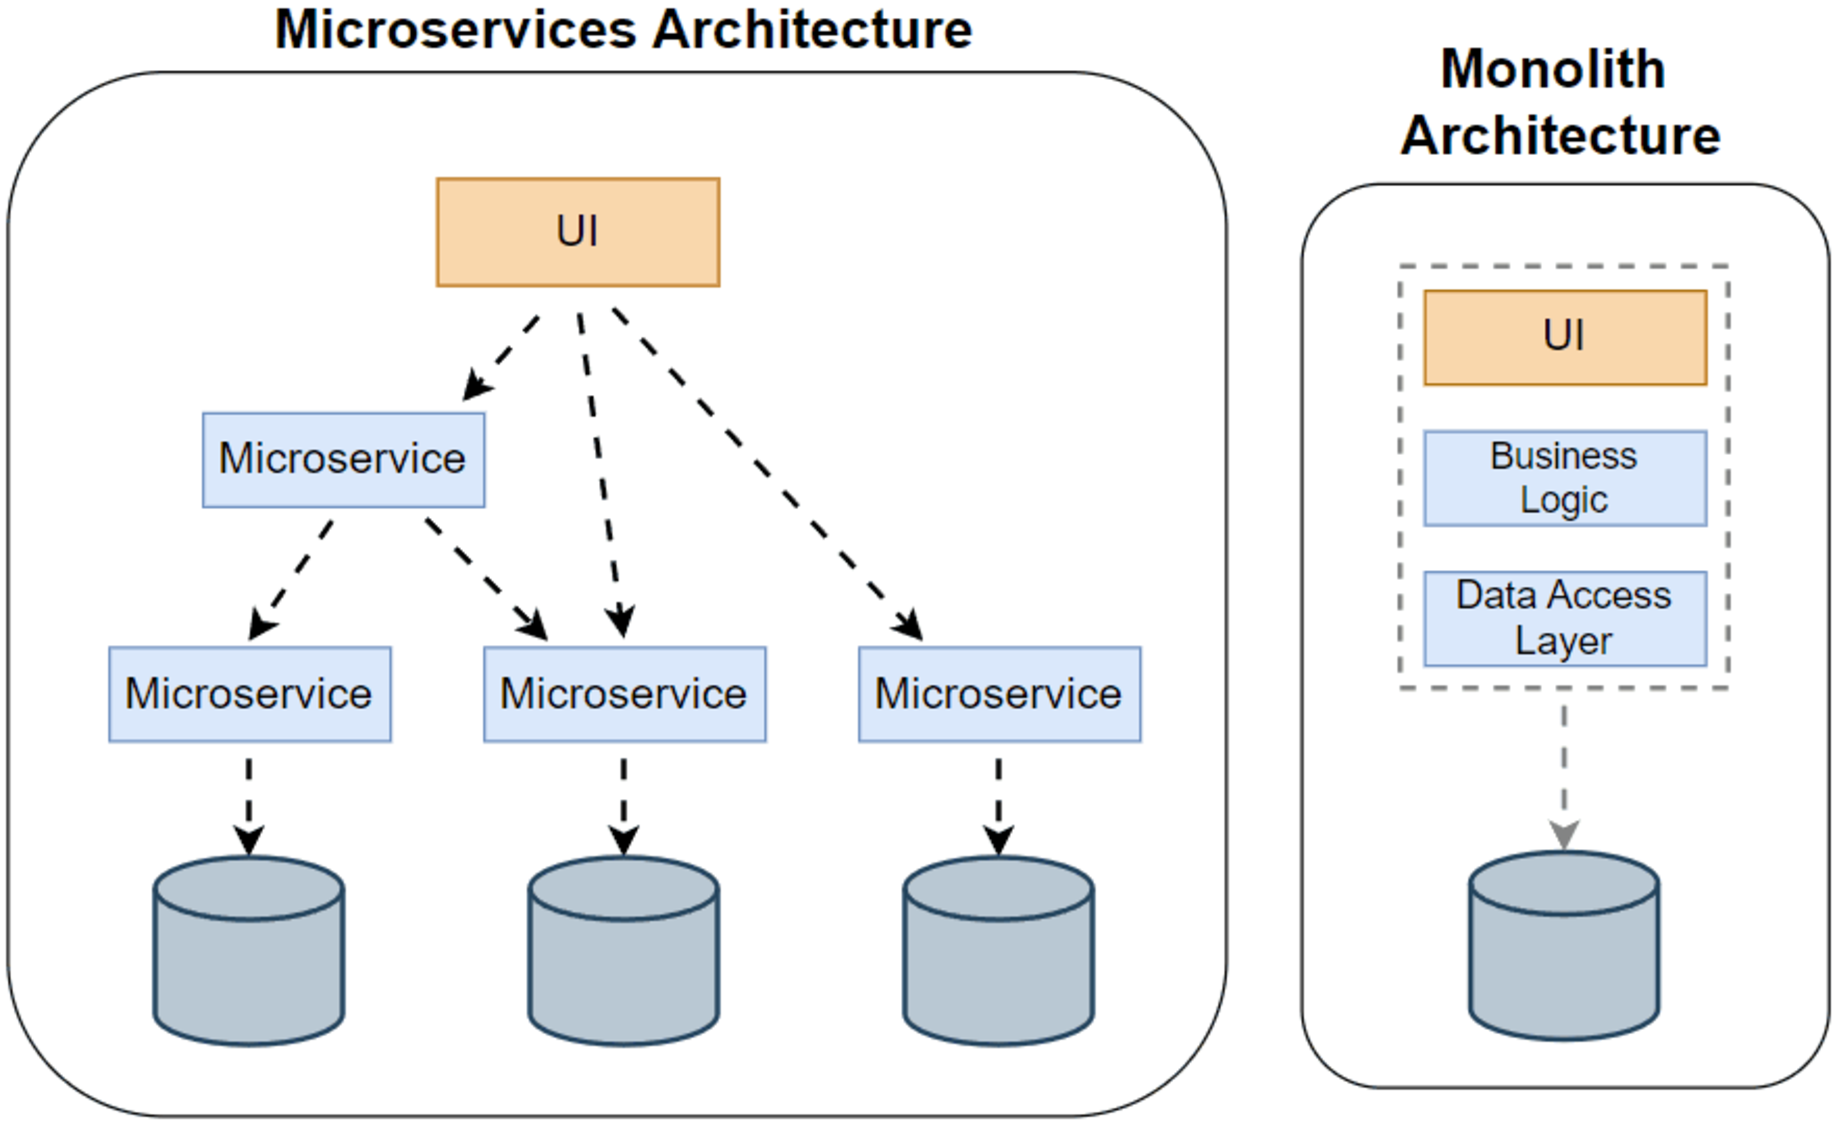
\includegraphics[width=0.95\textwidth]{images/architecture/microservices.pdf}
    \caption{Porównanie architektury monolitycznej i mikroserwisowej. Źródło:~\cite{blockbyte_microservices}}
    \label{fig:chapter2-monolith-vs-microservices}
\end{figure}

\subsection{Zalety i wady architektury monolitycznej}
\label{subsec:monolith-pros-cons}

Do najczęściej wskazywanych zalet architektury monolitycznej należy prostota implementacyjna i operacyjna. Jeden artefakt wdrożeniowy oznacza mniejszą liczbę komponentów do utrzymania, prostsze budowanie środowisk testowych oraz łatwiejszą konfigurację monitoringu, logowania i bezpieczeństwa. W projektach o ograniczonej skali przekłada się to na krótszy czas dostarczenia działającego rozwiązania oraz niższy koszt wejścia infrastrukturalnego \cite{villamizar2017cost,papakonstantinou2020technoeconomic,tapia2020monolithic,mangwani2023evaluation}.

Kolejną zaletą jest niski narzut komunikacyjny. Ponieważ współpraca między modułami aplikacji odbywa się lokalnie, system unika kosztów charakterystycznych dla rozproszonych architektur, takich jak opóźnienia sieciowe, serializacja wiadomości czy konieczność obsługi częściowych awarii. Badania porównawcze wskazują, że w scenariuszach bazujących na intensywnym wywoływaniu zależnych operacji monolit często uzyskuje lepsze czasy odpowiedzi i mniejszą latencję niż jego odpowiednik mikroserwisowy \cite{tapia2020monolithic,blinowski2022monolithic,okroj2023differences,bernsteiner2025performance}.

Do zalet należy także większa prostota testowania integracyjnego i lokalnego debugowania. Ponieważ wszystkie komponenty działają w ramach jednego procesu, łatwiejsze jest odtworzenie pełnego scenariusza wykonania, analiza stanu aplikacji oraz śledzenie przepływu danych. W małych i średnich systemach może to istotnie obniżyć koszt rozwoju i utrzymania \cite{benavente2022comparative,nayim2023ecommerce,berry2024migrating}.

Architektura monolityczna ma jednak również istotne ograniczenia. Najczęściej wskazywanym problemem jest trudność skalowania selektywnego. Przy wzroście obciążenia jednej części systemu konieczne bywa zwiększenie zasobów lub liczby instancji całej aplikacji, mimo że pozostałe moduły nie wymagają dodatkowej mocy obliczeniowej. Powoduje to mniej efektywne wykorzystanie infrastruktury i może prowadzić do wyższych kosztów przy nierównomiernym profilu obciążenia \cite{villamizar2017cost,papakonstantinou2020technoeconomic,blinowski2022monolithic,okroj2023differences}.

Drugim ograniczeniem jest rosnące sprzężenie wewnętrzne. Wraz z rozwojem systemu zwiększa się liczba zależności pomiędzy modułami, co utrudnia izolowanie zmian oraz podnosi koszt refaktoryzacji. W efekcie aplikacja monolityczna może stopniowo tracić elastyczność rozwojową, a wdrażanie nowych funkcji staje się coraz bardziej ryzykowne organizacyjnie i technicznie \cite{tapia2020monolithic,mangwani2023evaluation,berry2024migrating,kader2025streaming}.

Wadą bywa również mniejsza odporność na lokalne awarie logiczne. Błąd w krytycznej części aplikacji może wpływać na działanie całego systemu, ponieważ granice izolacji komponentów są słabsze niż w rozwiązaniach opartych na osobnych usługach. Problem ten staje się szczególnie istotny w systemach o dużej liczbie funkcji i wysokich wymaganiach dostępności \cite{blinowski2022monolithic,nayim2023ecommerce,berry2024migrating}.

\section{Architektura mikroserwisowa}
\label{sec:microservices-architecture}

Architektura mikroserwisowa zakłada budowę systemu jako zbioru niewielkich, autonomicznych usług realizujących wyodrębnione odpowiedzialności biznesowe. Każda usługa posiada własny cykl życia, może być wdrażana niezależnie i komunikuje się z pozostałymi komponentami za pomocą jawnie zdefiniowanych interfejsów. W praktyce oznacza to przejście od jednego centralnego artefaktu do układu wielu usług współtworzących logicznie spójny system \cite{tapia2020monolithic,blinowski2022monolithic,benavente2022comparative,adrio2023graphql,rashmi2024synthetic}.

Mikroserwisy są zwykle rozpatrywane w kontekście systemów chmurowych i kontenerowych, ponieważ takie środowiska ułatwiają ich wdrażanie, skalowanie oraz odtwarzanie po awarii. Literatura wskazuje jednak, że sama dekompozycja aplikacji nie gwarantuje automatycznie poprawy jakości systemu. Korzyści z mikroserwisów zależą od trafności podziału domenowego, liczby wywołań między usługami, sposobu utrzymania danych oraz właściwie dobranej technologii komunikacyjnej \cite{fontanadenardin2021energy,blinowski2022monolithic,okroj2023differences,rashmi2024synthetic,bernsteiner2025performance}.

\subsection{Cechy charakterystyczne architektury mikroserwisowej}
\label{subsec:microservices-characteristics}

Podstawową cechą architektury mikroserwisowej jest autonomia usług. Oznacza ona, że pojedynczy serwis posiada wydzielony zakres odpowiedzialności, własny interfejs oraz możliwość niezależnego wdrażania i rozwijania. W dobrze zaprojektowanym systemie zmiana implementacyjna jednej usługi nie powinna wymuszać zmian w pozostałych komponentach, o ile kontrakt komunikacyjny pozostaje stabilny \cite{blinowski2022monolithic,benavente2022comparative,mangwani2023evaluation,rashmi2024synthetic}.

Drugą istotną cechą jest rozproszenie komunikacji. Operacje, które w monolicie realizowane są lokalnie, w architekturze mikroserwisowej wymagają przesyłania danych przez sieć. Pojawiają się więc zagadnienia związane z kontraktami API, serializacją danych, czasem odpowiedzi, odpornością na błędy częściowe oraz obserwowalnością przepływu żądań pomiędzy usługami \cite{tapia2020monolithic,castillorivas2021performance,blinowski2022monolithic,berry2024migrating,bernsteiner2025performance}.

Trzecią cechą jest możliwość niezależnego skalowania usług. Jeżeli określony komponent systemu staje się wąskim gardłem, można zwiększyć liczbę jego instancji bez konieczności replikowania wszystkich pozostałych elementów aplikacji. Tego rodzaju elastyczność bywa wskazywana jako jedna z głównych przesłanek wyboru architektury mikroserwisowej w systemach działających przy zmiennym obciążeniu \cite{fontanadenardin2021energy,blinowski2022monolithic,mangwani2022container,okroj2023differences,kader2025streaming}.

Na rysunku~\ref{fig:chapter2-client-apps-gateway} pokazano przykładowy układ klientów, warstwy gateway i niezależnych usług biznesowych z osobnymi magazynami danych. Tego rodzaju schemat dobrze obrazuje logikę systemu rozproszonego, w którym punkt wejścia koordynuje dostęp do wielu autonomicznych komponentów.

\begin{figure}[htbp]
    \centering
    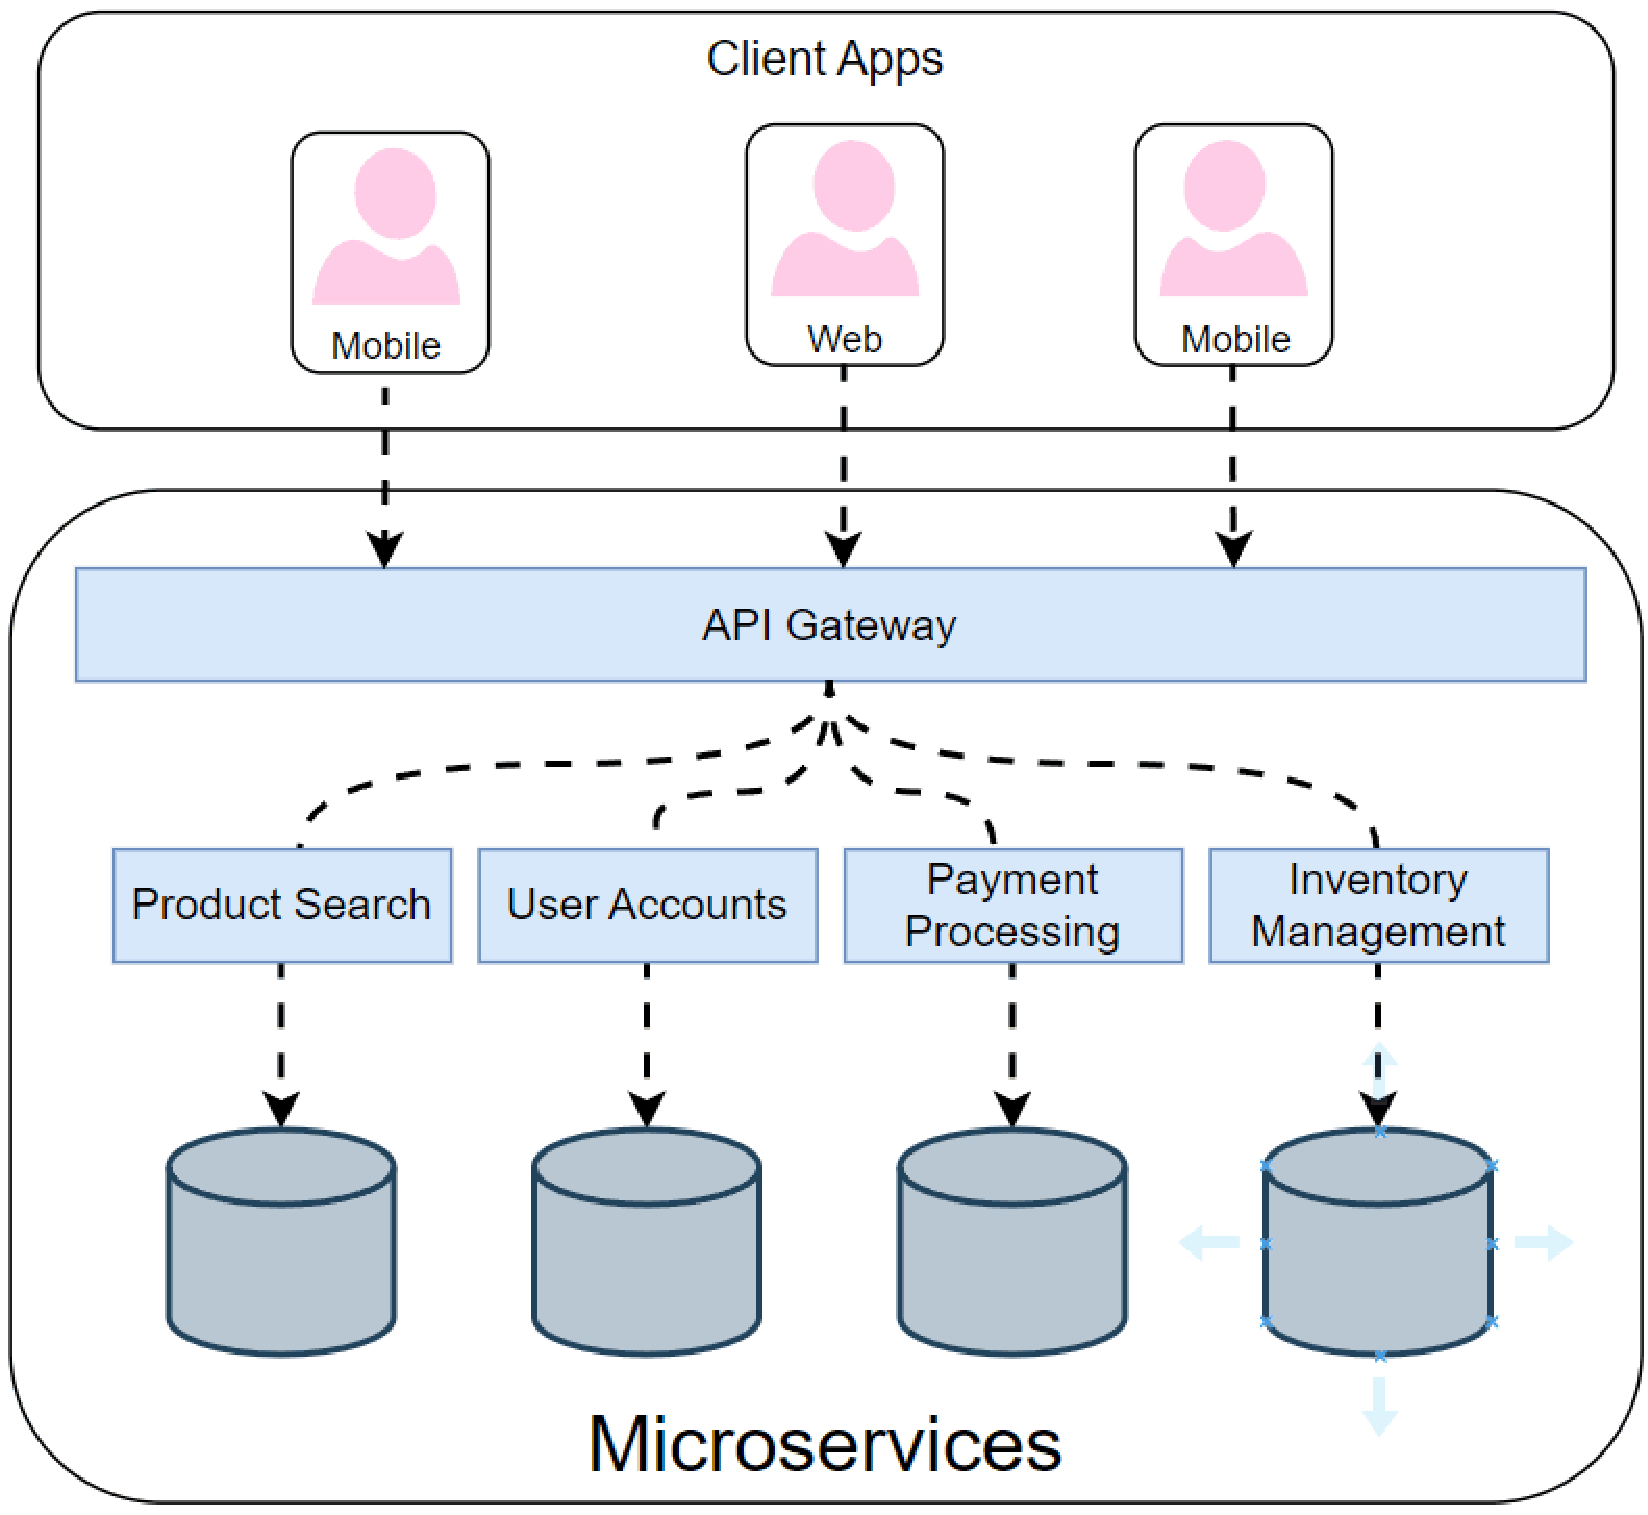
\includegraphics[width=0.92\textwidth]{images/architecture/client_apps}
    \caption{Przykładowy układ klientów, warstw i usług w architekturze mikroserwisowej. Źródło:~\cite{blockbyte_microservices}}
    \label{fig:chapter2-client-apps-gateway}
\end{figure}

\subsection{Zalety i wady architektury mikroserwisowej}
\label{subsec:microservices-pros-cons}

Najczęściej wskazywaną zaletą mikroserwisów jest elastyczność skalowania. Zamiast zwiększać zasoby całej aplikacji, można skalować tylko tę usługę, która rzeczywiście znajduje się pod największym obciążeniem. W środowiskach chmurowych pozwala to lepiej dopasować zużycie zasobów do aktualnego zapotrzebowania i w wielu scenariuszach może prowadzić do bardziej efektywnej eksploatacji infrastruktury \cite{villamizar2017cost,fontanadenardin2021energy,mangwani2022container,okroj2023differences,kader2025streaming}.

Drugą zaletą jest niezależność rozwojowa i wdrożeniowa. Mniejsze, autonomiczne usługi są łatwiejsze do refaktoryzacji i mogą być rozwijane przez różne zespoły równolegle. Przy zachowaniu odpowiednich kontraktów komunikacyjnych możliwe staje się częstsze wdrażanie zmian, a ewentualne problemy można ograniczać do pojedynczych komponentów zamiast całego systemu \cite{benavente2022comparative,mangwani2023evaluation,adrio2023graphql,rashmi2024synthetic}.

Do zalet zalicza się także możliwość lepszego dopasowania technologii do konkretnych zadań. W architekturze mikroserwisowej różne usługi mogą zostać zaimplementowane w odmiennych językach lub frameworkach, jeśli przynosi to korzyści funkcjonalne lub wydajnościowe. Podejście to zwiększa swobodę projektową, ale równocześnie wymaga większej dojrzałości organizacyjnej i operacyjnej \cite{papakonstantinou2020technoeconomic,blinowski2022monolithic,mangwani2023evaluation,rashmi2024synthetic}.

Najważniejszą wadą architektury mikroserwisowej jest wzrost złożoności systemu. Rozproszenie usług powoduje konieczność zarządzania wieloma procesami, konfiguracjami, wdrożeniami, kanałami komunikacji oraz mechanizmami obserwowalności. W praktyce system staje się trudniejszy do uruchomienia, monitorowania i diagnozowania niż aplikacja monolityczna \cite{papakonstantinou2020technoeconomic,castillorivas2021performance,okroj2023differences,berry2024migrating}.

Drugim kluczowym ograniczeniem jest narzut komunikacyjny. Każde zdalne wywołanie oznacza koszt transmisji, serializacji i oczekiwania na odpowiedź. Jeżeli architektura zostanie nadmiernie rozdrobniona, liczba wywołań między usługami może istotnie pogorszyć czas odpowiedzi i zwiększyć wrażliwość systemu na błędy częściowe. W wielu badaniach empirycznych wskazano, że poprawa skalowalności mikroserwisów nie zawsze idzie w parze z poprawą wydajności dla pojedynczego żądania \cite{tapia2020monolithic,blinowski2022monolithic,okroj2023differences,bernsteiner2025performance}.

Wadą są także wyższe wymagania dotyczące testowania i utrzymania spójności danych. W systemie rozproszonym trzeba uwzględnić nie tylko poprawność pojedynczych usług, ale również niezawodność całego łańcucha wywołań, zgodność kontraktów oraz odporność na awarie częściowe. Koszt ten rośnie wraz z liczbą usług, zależności i środowisk uruchomieniowych \cite{benavente2022comparative,mangwani2023evaluation,berry2024migrating,rashmi2024synthetic}.

\subsection{Metody komunikacji między mikroserwisami}
\label{subsec:microservices-communication}

Komunikacja między mikroserwisami może być realizowana w sposób synchroniczny lub asynchroniczny. W modelu synchronicznym jedna usługa wywołuje drugą i oczekuje na odpowiedź, co upraszcza model przepływu sterowania, ale zwiększa zależność czasową między komponentami. W modelu asynchronicznym wymiana danych odbywa się przez wiadomości, kolejki lub zdarzenia, co poprawia luźne sprzężenie, lecz utrudnia śledzenie przepływu i wymaga dodatkowych mechanizmów zapewniania spójności \cite{papakonstantinou2020technoeconomic,castillorivas2021performance,berry2024migrating,rashmi2024synthetic}.

Z punktu widzenia niniejszej pracy kluczowe znaczenie ma komunikacja synchroniczna oparta na gRPC~\cite{grpcdocs}. gRPC jest frameworkiem typu RPC wykorzystującym protokół HTTP/2 oraz binarną serializację Protocol Buffers. W praktyce umożliwia to definiowanie jednoznacznych, silnie typowanych kontraktów pomiędzy usługami oraz ograniczenie narzutu związanego z transmisją danych w porównaniu do formatów tekstowych, takich jak JSON. W efekcie komunikacja między usługami może być realizowana szybciej, przy mniejszym zużyciu zasobów oraz bardziej przewidywalnym czasie odpowiedzi~\cite{castillorivas2021performance,adrio2023graphql,berry2024migrating,bernsteiner2025performance}.

Schemat działania gRPC przedstawiono na rysunku~\ref{fig:grpc-digaram}.

\begin{figure}[htbp]
    \centering
    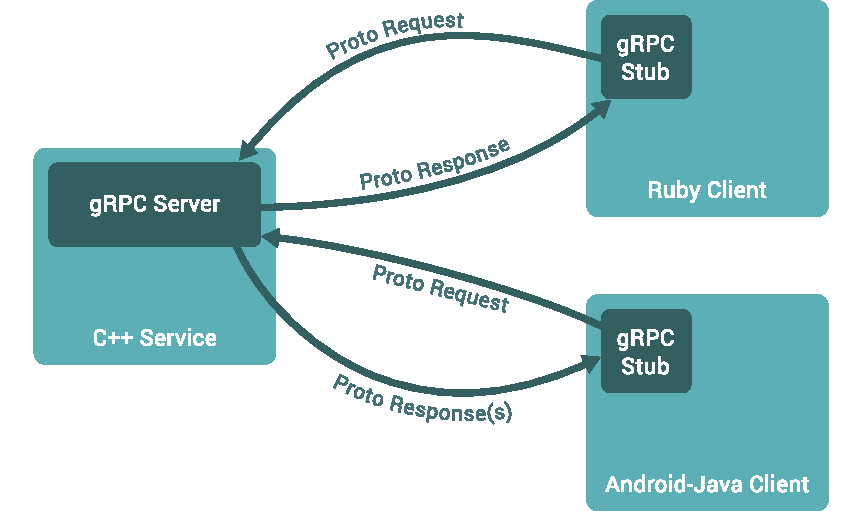
\includegraphics[width=0.92\textwidth]{images/architecture/grpc-diagram}
    \caption{Przykład komunikacji w modelu gRPC. Źródło:~\cite{grpcdocs}}
    \label{fig:grpc-digaram}
\end{figure}

W modelu tym klient nie komunikuje się bezpośrednio z implementacją usługi, lecz wykorzystuje wygenerowany na podstawie definicji interfejsu stub, który odpowiada za serializację żądania do formatu Protocol Buffers oraz obsługę komunikacji sieciowej. Żądanie (Proto Request) przesyłane jest do serwera gRPC, który udostępnia implementację logiki biznesowej, a następnie zwraca odpowiedź (Proto Response). Jak pokazano na rysunku, ten sam serwer może obsługiwać wielu klientów zaimplementowanych w różnych językach programowania (np. Ruby czy Java), co podkreśla wielojęzyczny charakter gRPC oraz jego przydatność w środowiskach niejednolitych implementacyjnie. :contentReference[oaicite:0]{index=0}


Ważną właściwością gRPC jest również wsparcie dla różnych modeli wywołań, w tym wywołań jednokrotnych (unary) oraz komunikacji strumieniowej. Umożliwia to dostosowanie sposobu komunikacji do charakteru przetwarzanych danych, np. w scenariuszach wymagających przesyłania wielu odpowiedzi lub ciągłego strumienia danych. Dodatkowo wykorzystanie plików definicji interfejsów pozwala generować kod klientów i serwerów w wielu językach programowania, co dobrze współgra z heterogenicznym środowiskiem technologicznym i zróżnicowanymi implementacjami usług~\cite{adrio2023graphql,rashmi2024synthetic,berry2024migrating}.

Z drugiej strony wybór gRPC nie eliminuje fundamentalnych problemów architektury rozproszonej. Nadal występują opóźnienia sieciowe, ryzyko przekroczenia limitów czasowych (timeouts), błędy częściowe oraz konieczność monitorowania komunikacji między usługami. Ostateczna wydajność systemu zależy więc nie tylko od zastosowanego protokołu, lecz również od liczby wywołań między usługami, wielkości komunikatów, charakterystyki obciążenia oraz jakości podziału systemu na mikroserwisy~\cite{tapia2020monolithic,blinowski2022monolithic,okroj2023differences,bernsteiner2025performance}.

W literaturze podkreśla się również znaczenie rozważnego doboru liczby usług i granic odpowiedzialności. Nadmierna granularność może prowadzić do sytuacji, w której koszty komunikacji i koordynacji przewyższają korzyści wynikające z modularności. Z kolei zbyt szerokie granice serwisów ograniczają potencjał niezależnego skalowania i osłabiają korzyści wynikające z dekompozycji \cite{blinowski2022monolithic,okroj2023differences,berry2024migrating,kader2025streaming}.

\section{Skalowalność i wydajność systemów rozproszonych}
\label{sec:scalability-performance}

Wydajność i skalowalność należą do najczęściej analizowanych właściwości w badaniach porównujących monolity i mikroserwisy. Wydajność jest zwykle opisywana za pomocą takich metryk jak czas odpowiedzi, latencja, przepustowość czy wykorzystanie zasobów. Skalowalność odnosi się natomiast do zdolności systemu do utrzymania akceptowalnego poziomu jakości usług przy wzroście obciążenia oraz do efektywnego wykorzystania dodatkowych zasobów obliczeniowych \cite{tapia2020monolithic,blinowski2022monolithic,okroj2023differences,nayim2023ecommerce,bernsteiner2025performance}.

W systemach rozproszonych na wynik wydajnościowy wpływa przede wszystkim liczba zdalnych wywołań w ścieżce obsługi żądania. Każde dodatkowe wywołanie powoduje powstanie kosztu transportu danych, serializacji, kolejkowania i synchronizacji odpowiedzi. Jeżeli pojedyncze żądanie klienta uruchamia długi łańcuch zależnych wywołań, narzut ten może być istotny nawet wtedy, gdy poszczególne usługi są same w sobie szybkie \cite{tapia2020monolithic,castillorivas2021performance,blinowski2022monolithic,bernsteiner2025performance}.

Jednocześnie architektura mikroserwisowa może przewyższać monolit pod względem skalowalności poziomej, szczególnie gdy wąskie gardła systemu są skoncentrowane w niewielkiej liczbie usług. W takim przypadku można zwiększyć liczbę instancji tylko tych komponentów, które rzeczywiście wymagają dodatkowej mocy obliczeniowej, bez konieczności replikowania całego systemu. Badania pokazują jednak, że przewaga ta jest silnie zależna od scenariusza obciążenia oraz sposobu dekompozycji aplikacji \cite{fontanadenardin2021energy,mangwani2022container,okroj2023differences,mangwani2023evaluation,kader2025streaming}.

W praktyce architektura rozproszona wprowadza również nowe klasy ograniczeń wydajnościowych. Należą do nich m.in. koszty balansowania obciążenia, przełączania kontekstu pomiędzy usługami, agregowania danych z wielu źródeł czy utrzymywania dodatkowych warstw pośrednich. Oznacza to, że mikroserwisy mogą uzyskać lepsze zachowanie pod rosnącym obciążeniem, a jednocześnie mieć gorszy czas odpowiedzi dla pojedynczego wywołania niż porównywalny monolit \cite{blinowski2022monolithic,okroj2023differences,berry2024migrating,bernsteiner2025performance}.

Warto również zauważyć, że skalowalność nie jest cechą wyłącznie architektury, lecz całego układu: implementacji, sposobu wdrożenia, konfiguracji kontenerów, algorytmów równoważenia obciążenia oraz charakterystyki danych wejściowych. Z tego powodu wyniki badań eksperymentalnych często różnią się między sobą, a przewaga jednego podejścia nad drugim ma charakter warunkowy, a nie absolutny \cite{tapia2020monolithic,blinowski2022monolithic,rashmi2024synthetic,berry2024migrating,kader2025streaming}.

\section{Koszty utrzymania aplikacji w środowiskach chmurowych}
\label{sec:cloud-maintenance-costs}

Koszty utrzymania aplikacji w środowiskach chmurowych obejmują znacznie więcej niż bezpośrednie opłaty za procesor, pamięć operacyjną czy transfer danych. W ujęciu praktycznym należy uwzględnić również koszt wdrożeń, monitoringu, logowania, orkiestracji, utrzymania pipeline'ów CI/CD, zarządzania konfiguracją, reagowania na incydenty oraz koszt pracy zespołów odpowiedzialnych za rozwój i operacyjne utrzymanie systemu \cite{villamizar2017cost,papakonstantinou2020technoeconomic,fontanadenardin2021energy,okroj2023differences,berry2024migrating}.

W architekturze monolitycznej koszty początkowe bywają niższe, ponieważ system składa się z mniejszej liczby komponentów i wymaga prostszej infrastruktury pomocniczej. Wdrożenie jednego artefaktu, centralne logowanie i jednolite środowisko wykonawcze upraszczają zarówno konfigurację, jak i codzienne utrzymanie. W małych i średnich systemach może to oznaczać realnie niższy całkowity koszt eksploatacji \cite{villamizar2017cost,papakonstantinou2020technoeconomic,mangwani2023evaluation,nayim2023ecommerce}.

Z kolei architektura mikroserwisowa może przynosić korzyści kosztowe wtedy, gdy niezależne skalowanie usług rzeczywiście pozwala ograniczyć nadmiarową alokację zasobów. Jeżeli tylko niewielka część systemu wymaga dużej mocy obliczeniowej, selektywne skalowanie może okazać się bardziej opłacalne niż zwiększanie zasobów całej aplikacji monolitycznej. Tego rodzaju efekty były raportowane w badaniach analizujących koszty architektur chmurowych oraz elastyczność wykorzystania infrastruktury \cite{villamizar2017cost,fontanadenardin2021energy,okroj2023differences,kader2025streaming}.

Potencjalne korzyści kosztowe mikroserwisów są jednak równoważone przez wzrost złożoności operacyjnej. Większa liczba usług oznacza więcej kontenerów, definicji wdrożeniowych, metryk, dashboardów, reguł alarmowych i potencjalnych punktów awarii. Koszty te nie zawsze są widoczne w prostych kalkulacjach infrastrukturalnych, ale w praktyce mają istotny wpływ na całkowity koszt utrzymania systemu \cite{papakonstantinou2020technoeconomic,castillorivas2021performance,okroj2023differences,berry2024migrating}.

W literaturze zwraca się także uwagę na koszt energetyczny i efektywność wykorzystania zasobów. W środowiskach rozproszonych dodatkowa warstwa komunikacji i większa liczba procesów mogą powodować wzrost zużycia energii, nawet jeśli architektura oferuje korzystniejsze właściwości skalowania. Z tego względu ocena kosztów powinna obejmować nie tylko wydajność czysto infrastrukturalną, ale również efektywność energetyczną oraz nakład operacyjny potrzebny do utrzymania systemu w stabilnym stanie \cite{fontanadenardin2021energy,berry2024migrating}.

Z perspektywy decyzji architektonicznej kluczowe jest więc przyjęcie szerokiego rozumienia kosztu. Wybór pomiędzy monolitem a mikroserwisami nie powinien opierać się wyłącznie na cenie uruchomienia pojedynczej instancji, lecz na całościowym bilansie obejmującym wydajność, elastyczność skalowania, złożoność operacyjną oraz koszty organizacyjne \cite{villamizar2017cost,papakonstantinou2020technoeconomic,okroj2023differences,berry2024migrating,bernsteiner2025performance}.

\section{Podsumowanie}
\label{sec:chapter2-summary}

Architektura monolityczna i mikroserwisowa reprezentują dwa odmienne sposoby organizacji systemu, z których każdy prowadzi do innego rozkładu korzyści i kosztów. Monolit oferuje prostszy model wdrożeniowy, mniejszy narzut komunikacyjny i zwykle niższy koszt początkowy, lecz wraz ze wzrostem systemu może tracić elastyczność skalowania i zwiększać trudność rozwoju. Mikroserwisy zapewniają większą modularność, możliwość niezależnego skalowania oraz lepsze dopasowanie do środowisk chmurowych, ale osiągają te korzyści kosztem wyższej złożoności operacyjnej i dodatkowego narzutu komunikacyjnego \cite{tapia2020monolithic,blinowski2022monolithic,okroj2023differences,berry2024migrating,bernsteiner2025performance}.

Dla dalszej części pracy szczególnie istotne są dwa wnioski. Po pierwsze, przewaga mikroserwisów nad monolitem nie jest bezwarunkowa, lecz zależy od scenariusza obciążenia, trafności dekompozycji systemu oraz sposobu komunikacji między usługami. Po drugie, w przypadku architektury mikroserwisowej wybór technologii komunikacyjnej, w tym gRPC, ma realny wpływ na wynik końcowy zarówno w obszarze wydajności, jak i złożoności utrzymania. Te obserwacje stanowią bezpośrednie uzasadnienie dla dalszych badań eksperymentalnych przeprowadzonych w niniejszej pracy \cite{castillorivas2021performance,adrio2023graphql,rashmi2024synthetic,berry2024migrating,bernsteiner2025performance}.